\subsection{Mesh generation}

\subsubsection{Selection of the tutorial}

\paragraph{}The selection of the tutorial case is the first thing that needs to be done to run the simulation of the turbofan since all the files that will be used are linked and, starting a new case would mean spending a lot of time creating files and establishing all these links in order to make \textit{OpenFOAM} work properly. Among all the tutorials that can be found on the \textit{OpenFOAM} folder, we have selected the \textit{mixerVesselAMI2D} for several reasons. 

\subsubsection{blockMesh}

\paragraph{}The definition of the \textit{blockMeshDict} is the first part that needs to be modified. The \textit{blockMesh} must contain the geometry that has to be simulated and we must have an idea of the vertices of the parallelogram that will contain the first stages of the compressor. In order to do that, the geometry has to be opened using either \textit{Salome} or \textit{Paraview}. Then the axes must be showed and the points have to be written down on the \textit{blockMesh} file.

\begin{figure}
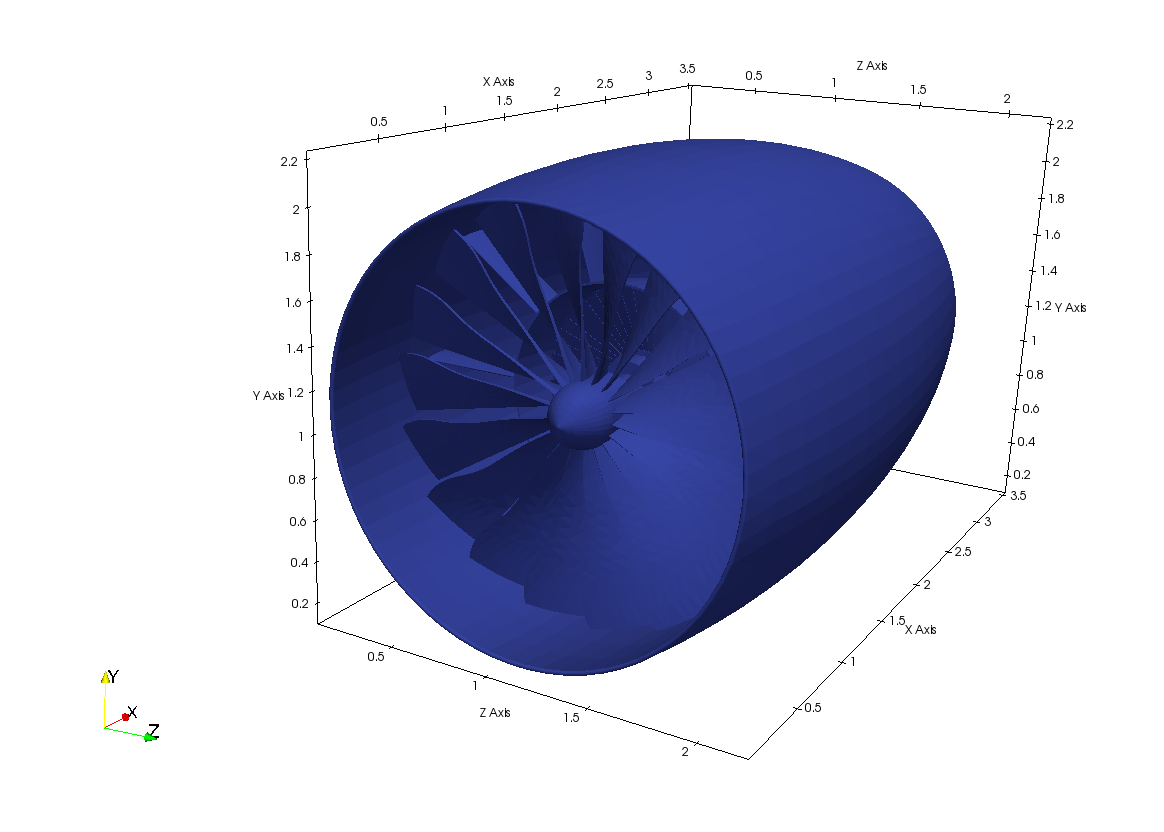
\includegraphics[scale=0.30]{./img/geometryAxes}
\centering
\caption{Turbofan with axes}
\label{axisparaview}
\end{figure}

\paragraph{}Now that the points enclosing the desired geometry are clear, they can be modified in the \textit{blockMeshDict} file. This change is presented below:

\begin{footnotesize}
\begin{verbatim}
vertices
(
    (0.77 0   0)
    (1.35 0   0)
    (1.35 2.3 0)
    (0.77 2.3 0)
    (0.77 0   2.3)
    (1.35 0   2.3)
    (1.35 2.3 2.3)
    (0.77 2.3 2.3)
);
\end{verbatim}
\end{footnotesize}

\paragraph{}It can be clearly seen that the domain of the mesh is a $0.58$x$2.3$x$2.3m$ rectangular prism.

\paragraph{}Once the boundaries of the \textit{blockMesh} are defined, the number of cells that it will have has to be set. It has to be taken into account that a very dense mesh at the beginning will not be efficient when simulating the case given that we will use the \textit{snappyHexMesh} later, so it might be over densified. On the other hand, a very coarse mesh will not be efficient either because additional divisions will have to be set when generating the refined mesh and the computational time of the \textit{snappyHexMesh} process might grow. Thus, a solution between a mesh with a very high number of cells and a very low number of cells has to be attained.

\paragraph{}This basic mesh has been divided every $0.05m$. It means that we have done 12 divisions in the x direction, 46 on the y direction and 46 more on the z direction. 

\begin{footnotesize}
\begin{verbatim}
blocks
(
    hex (0 1 2 3 4 5 6 7) (12 46 46) simpleGrading (1 1 1)
);
\end{verbatim}
\end{footnotesize}

\paragraph{}Finally, the differents faces of the mesh must be defined depending on whether they are the inlet or outlet faces or the lateral faces of the geometry.To do this, \textit{OpenFOAM} numbers the vertices according to their appearance in the \textit{blockMeshDict} and the faces are defined by four those numbers. Since the vertex numeration has been kept the same as the one that comes as default in every tutorial case; it is easier to define the inlet face of the \textit{blockMesh} (this is: the face in which the flow comes in) as well as the outlet face (this is: the face in which the flow comes out) that will be used to define the boundary conditions later.

\begin{footnotesize}
\begin{verbatim}
boundary
(
    frontAndBack
    {
        type patch;
        faces
        (
            (3 7 6 2)
            (1 5 4 0)
            (0 3 2 1)
            (4 5 6 7)
        );
    }
    inlet
    {
        type patch;
        faces
        (
            (0 4 7 3)
        );
    }
    outlet
    {
        type patch;
        faces
        (
            (2 6 5 1)
        );
    }
);
\end{verbatim}
\end{footnotesize}

\paragraph{}The \textit{blockMeshDict} file is presented below. This is the final file that has been used to generate the \textit{blockMesh} and it is included in the \textit{.zip} file attached to this report. Only the parameters mentioned above have been modified; the rest is equal to the tutorial case that has been selected.

\begin{footnotesize}
\begin{verbatim}
/*--------------------------------*- C++ -*----------------------------------*\
| =========                 |                                                 |
| \\      /  F ield         | OpenFOAM: The Open Source CFD Toolbox           |
|  \\    /   O peration     | Version:  4.0                                   |
|   \\  /    A nd           | Web:      www.OpenFOAM.org                      |
|    \\/     M anipulation  |                                                 |
\*---------------------------------------------------------------------------*/
FoamFile
{
    version     2.0;
    format      ascii;
    class       dictionary;
    object      blockMeshDict;
}

// * * * * * * * * * * * * * * * * * * * * * * * * * * * * * * * * * * * * * //

convertToMeters 1;

vertices
(
    (0.77 0   0)
    (1.35 0   0)
    (1.35 2.3 0)
    (0.77 2.3 0)
    (0.77 0   2.3)
    (1.35 0   2.3)
    (1.35 2.3 2.3)
    (0.77 2.3 2.3)
);

blocks
(
    hex (0 1 2 3 4 5 6 7) (12 46 46) simpleGrading (1 1 1)
);

edges
(
);

boundary
(
    frontAndBack
    {
        type patch;
        faces
        (
            (3 7 6 2)
            (1 5 4 0)
            (0 3 2 1)
            (4 5 6 7)
        );
    }
    inlet
    {
        type patch;
        faces
        (
            (0 4 7 3)
        );
    }
    outlet
    {
        type patch;
        faces
        (
            (2 6 5 1)
        );
    }
);

// ************************************************************************* //
\end{verbatim}
\end{footnotesize}

\paragraph{}The log obtained when the \textit{blockMesh} has been generated is presented below. As it can be seen, no errors were found during the computation of this basic mesh. The number of cells is relatively high (\textbf{25392}) but perfectly suitable to proceed with the refinement of the mesh. Additionally, a caption of the basic mesh is presented in \ref{blockMeshcaption}.


\begin{footnotesize}
\begin{verbatim}
/*---------------------------------------------------------------------------*\
| =========                 |                                                 |
| \\      /  F ield         | OpenFOAM: The Open Source CFD Toolbox           |
|  \\    /   O peration     | Version:  4.0                                   |
|   \\  /    A nd           | Web:      www.OpenFOAM.org                      |
|    \\/     M anipulation  |                                                 |
\*---------------------------------------------------------------------------*/
Build  : 4.0-665f1db4c1f1
Exec   : blockMesh
Date   : Dec 05 2016
Time   : 14:17:05
Host   : "victorPC"
PID    : 4499
Case   : /home/victor/Desktop/Final/pimpleDyMFoam/turbofan_std
nProcs : 1
sigFpe : Enabling floating point exception trapping (FOAM_SIGFPE).
fileModificationChecking : Monitoring run-time modified files using timeStampMaster
allowSystemOperations : Allowing user-supplied system call operations

// * * * * * * * * * * * * * * * * * * * * * * * * * * * * * * * * * * * * * //
Create time

Creating block mesh from
    "/home/victor/Desktop/Final/pimpleDyMFoam/turbofan_std/system/blockMeshDict"
Creating curved edges
Creating topology blocks
Creating topology patches

Creating block mesh topology

Check topology

	Basic statistics
		Number of internal faces : 0
		Number of boundary faces : 6
		Number of defined boundary faces : 6
		Number of undefined boundary faces : 0
	Checking patch -> block consistency

Creating block offsets
Creating merge list .

Creating polyMesh from blockMesh
Creating patches
Creating cells
Creating points with scale 1
    Block 0 cell size :
        i : 0.0483333 .. 0.0483333
        j : 0.05 .. 0.05
        k : 0.05 .. 0.05


There are no merge patch pairs edges

Writing polyMesh
----------------
Mesh Information
----------------
  boundingBox: (0.77 0 0) (1.35 2.3 2.3)
  nPoints: 28717
  nCells: 25392
  nFaces: 79396
  nInternalFaces: 72956
----------------
Patches
----------------
  patch 0 (start: 72956 size: 2208) name: frontAndBack
  patch 1 (start: 75164 size: 2116) name: inlet
  patch 2 (start: 77280 size: 2116) name: outlet

End
\end{verbatim}
\end{footnotesize}


\begin{figure}[h!]
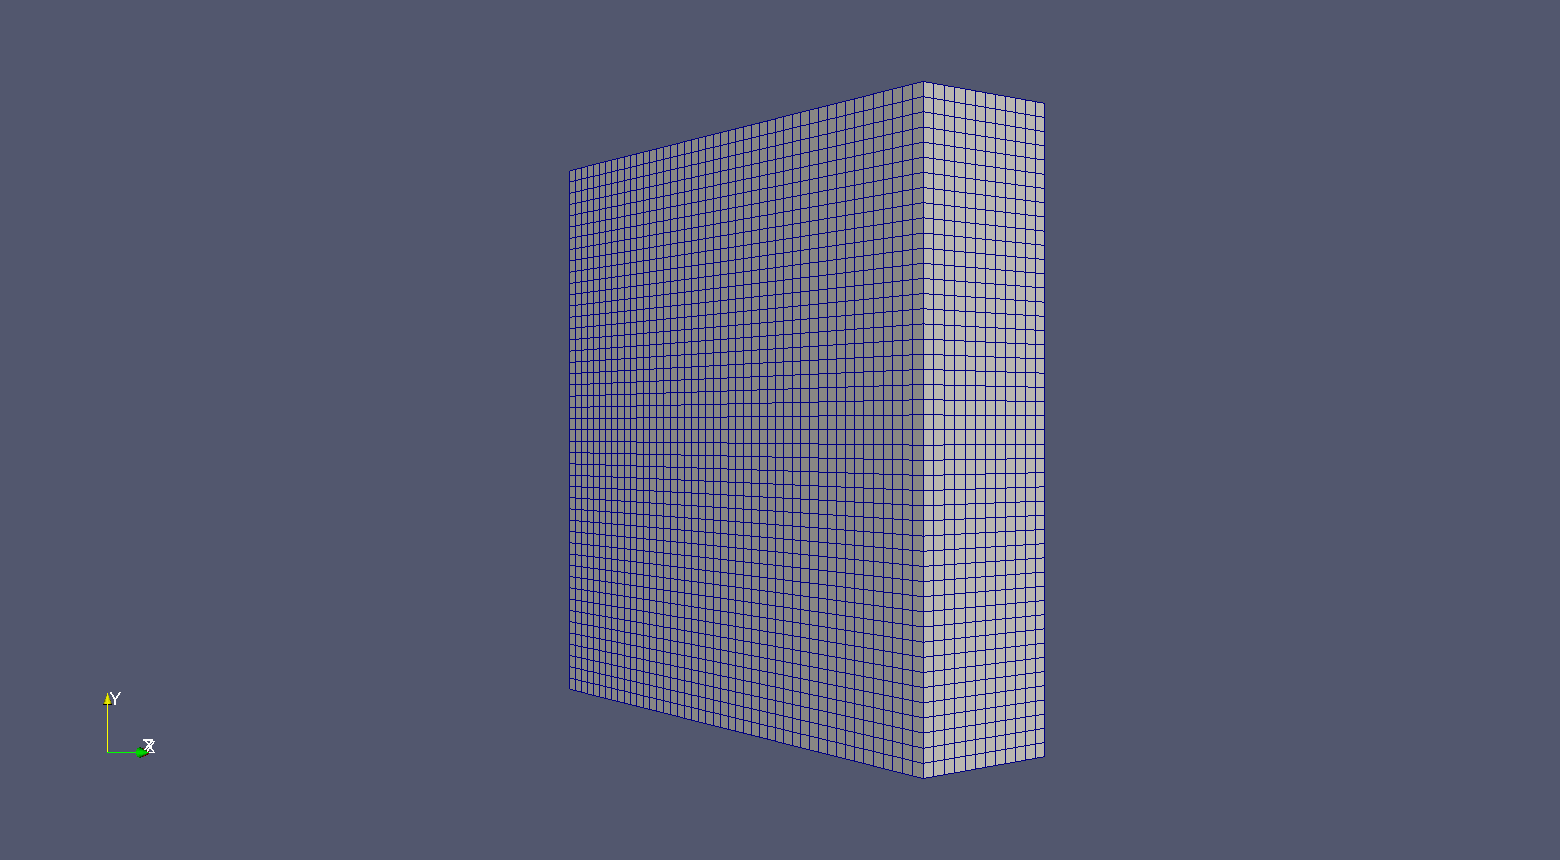
\includegraphics[scale=0.26]{./mesh/screenshots/blockmesh}
\centering
\caption{blockMeshcaption}
\label{blockMeshcaption}
\end{figure}

\subsubsection{Mesh refinement}

\paragraph{}To refine the mesh, the \textit{snappyHexMesh} utility is used (included in \textit{OpenFOAM}) and several parameters have to be modified in order to obtain a dense mesh that is suitable for the simulation of this complex geometry. It has to be considered that a particular geometry is has a relative velocity as well; this is, the rotor is rotating, and so the first and second stages of the Low Pressure Compression of the turbofan engine, while the nacelle and the combustor are static. 

\paragraph{}In the \textit{snappyHexMeshDict} several parameters have to be modified. First, the \textit{snappyHexMesh} must be aware of the geometries that it has to take into account. As it can be seen below, the files \textit{Fan.stl}, \textit{HPSpool.stl}, \textit{LPSpool.stl} and \textit{NacelleStator.stl} have been included here.

\begin{footnotesize}
\begin{verbatim}
geometry
{
    box1x1x1
    {
        type searchableBox;
        min (1.5 1 -0.5);
        max (3.5 2 0.5);
    }

    Fan.stl
    {
        type triSurfaceMesh;
        regions
        {
        }
    }
    HPSpool.stl
    {
        type triSurfaceMesh;
        regions
        {
        }
    }
    LPSpool.stl
    {
        type triSurfaceMesh;
        regions
        {
        }
    }
    NacelleStator.stl
    {
        type triSurfaceMesh;
        regions
        {
        }
    }
};
\end{verbatim}
\end{footnotesize}

\paragraph{}Next, the number of control volumes has to be limited to ensure that the laptop is capable of running a simulation. This number has been limited to two million cells, which is a pretty high number and the following lines have to be modified.

\begin{footnotesize}
\begin{verbatim}
    // Overall cell limit (approximately). Refinement will stop immediately
    // upon reaching this number so a refinement level might not complete.
    // Note that this is the number of cells before removing the part which
    // is not 'visible' from the keepPoint. The final number of cells might
    // actually be a lot less.
    maxGlobalCells 2000000;
\end{verbatim}
\end{footnotesize}

\paragraph{}The next step is to define the refinement required of the mesh for the different geometries that will be simulated. It can be clearly seen in this section that we have included the same \textit{STL} files that we did before. The higher the level of the refinement, the denser the mesh will be and the better it will resemble to the real geometry. But the limitation here is the computational power so, the maximum refinement number cannot be as high as we would like to. Thus, depending on the complexity of the geometry, several minimum (the first number) and maximum (the second number) refinement leves have been defined.

\begin{footnotesize}
\begin{verbatim}
    // Surface based refinement
    // ~~~~~~~~~~~~~~~~~~~~~~~~

    // Specifies two levels for every surface. The first is the minimum level,
    // every cell intersecting a surface gets refined up to the minimum level.
    // The second level is the maximum level. Cells that 'see' multiple
    // intersections where the intersections make an
    // angle > resolveFeatureAngle get refined up to the maximum level.

    refinementSurfaces
    {
        Fan.stl
        {
            // Surface-wise min and max refinement level
            level (3 5);

            // Optional region-wise level specification
            regions
            {
            }
            patchInfo
            {
                type patch;
                inGroups (meshedPatches);
            }
	}
        HPSpool.stl
        {
            // Surface-wise min and max refinement level
            level (3 5);

            // Optional region-wise level specification
            regions
            {
            }
            patchInfo
            {
                type patch;
                inGroups (meshedPatches);
            }
	}
        LPSpool.stl
        {
            // Surface-wise min and max refinement level
            level (6 8);
	    cellZone rotor; cellZoneInside inside;

            // Optional region-wise level specification
            regions
            {
            }
            patchInfo
            {
                type patch;
                inGroups (meshedPatches);
            }
	}
        NacelleStator.stl
        {
            // Surface-wise min and max refinement level
            level (4 6);

            // Optional region-wise level specification
            regions
            {
            }
            patchInfo
            {
                type patch;
                inGroups (meshedPatches);
            }
	}
    }
\end{verbatim}
\end{footnotesize}

\paragraph{}It is worth mentioning that a zone has been defined within  the \textit{LPSpool.stl} of the surface refinement from above. The MFR options must have a particular set of cellzones defined that will rotate. So, in order to make these first stages of the compressor to rotate, this has to be defined.

\begin{footnotesize}
\begin{verbatim}
        LPSpool.stl
        {
            // Surface-wise min and max refinement level
            level (6 8);
	    cellZone rotor; cellZoneInside inside;
		[...] %MODIFIED ^
\end{verbatim}
\end{footnotesize}


\paragraph{}The next step is to select a point within the mesh. So, the \textit{locationInMesh} has to be modified with the x, y, and z-coordinates of a point with that feature.

\begin{footnotesize}
\begin{verbatim}
    // After refinement patches get added for all refinementSurfaces and
    // all cells intersecting the surfaces get put into these patches. The
    // section reachable from the locationInMesh is kept.
    // NOTE: This point should never be on a face, always inside a cell, even
    // after refinement.
    locationInMesh (.97443222 1.40534444343 1.24221211);
\end{verbatim}
\end{footnotesize}

\paragraph{}Finally, the \textit{surfaceFeatureExtract} has been used.  What this option does it to refine even more the mesh near the points that have complex geometries such as the edges of the blades. This is particularly useful for the turbofan given that it has a high number of blades and a twisting geometry that will resemble more to the reality when using this option. Thus, the following lines within the \textit{snappyHexMeshDict} must be modified.

\begin{footnotesize}
\begin{verbatim}
   // Explicit feature edge refinement
    // ~~~~~~~~~~~~~~~~~~~~~~~~~~~~~~~~

    // Specifies a level for any cell intersected by explicitly provided
    // edges.
    // This is a featureEdgeMesh, read from constant/triSurface for now.
    // Specify 'levels' in the same way as the 'distance' mode in the
    // refinementRegions (see below). The old specification
    //      level   2;
    // is equivalent to
    //      levels  ((0 2));

    features
    (
        {
           file "NacelleStator.eMesh";
           level 5;
        //    levels ((0.0 2) (1.0 3));
        }
        {
           file "LPSpool.eMesh";
           level 7;
        //    levels ((0.0 2) (1.0 3));
        }
    );
\end{verbatim}
\end{footnotesize}

\paragraph{}All of the other parameters of the \textit{snappyHexMeshDict} have not been modified.

\subsubsection{Comparison of different types of mesh}


\paragraph{}A comparison between the coarse mesh and the refined mesh generated is presented below. The mesh that has been used to simulate the case is the refined mesh (for obvious reasons). Also, it has to be kept in mind that the coarser the mesh, the worse that the geometry will be (this is, it will not resemble to the real geometry), as can be seen below.

\newpage\subsubsubsection{Coarse mesh}

\paragraph{}The number of control volumes in the mesh is 40, which is a very small number given the size of the turbofan. It can be seen in \ref{coarse1} and \ref{coarse2} that this mesh cannot be used to run a simulation.

\begin{figure}[h!]
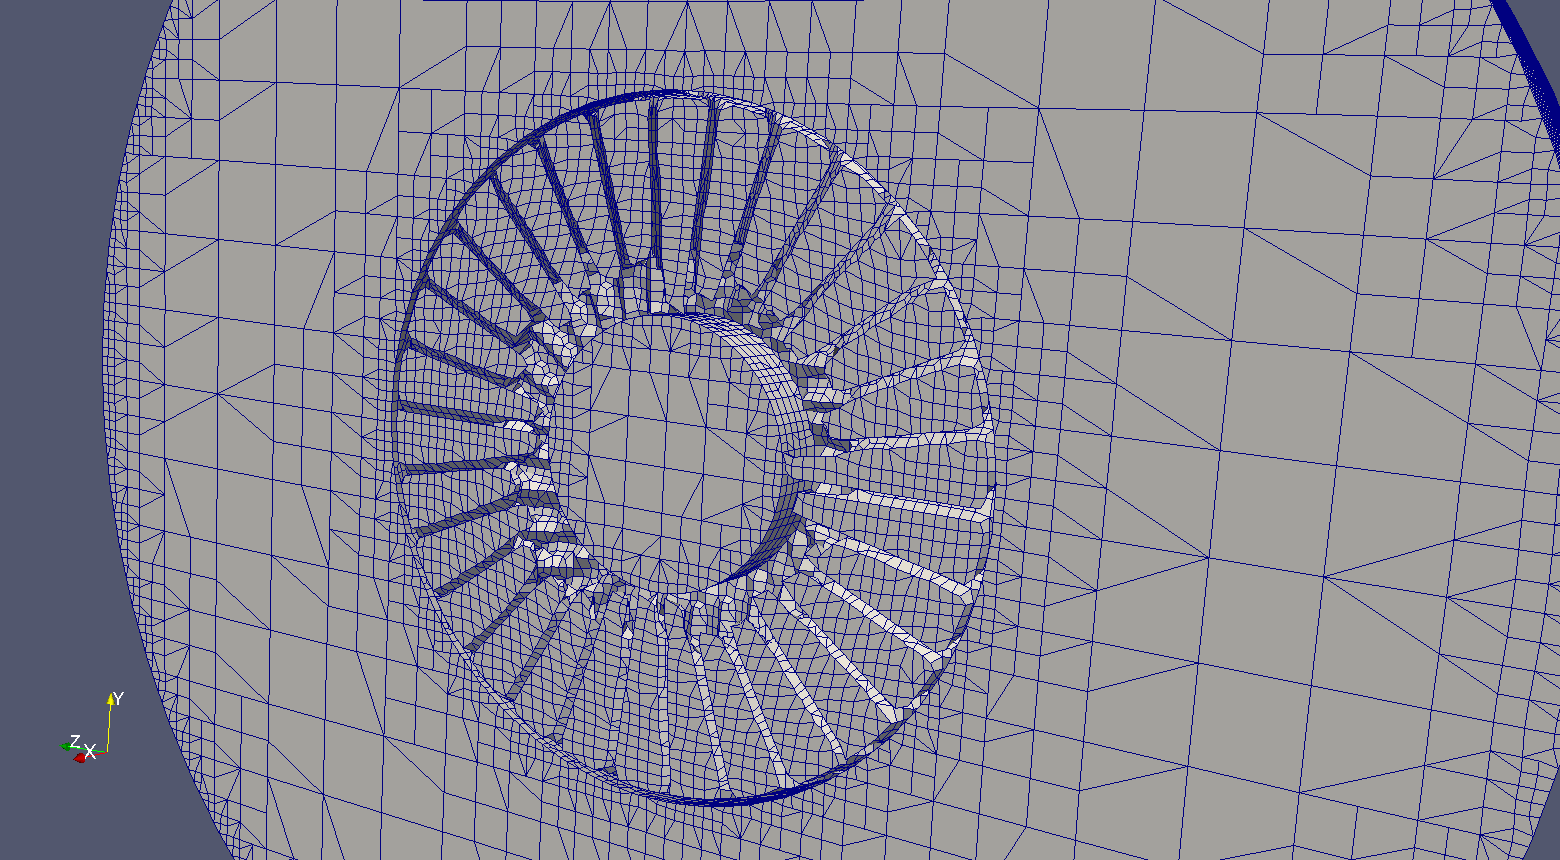
\includegraphics[scale=0.24]{./mesh/screenshots/coarse2}
\centering
\caption{Detail of the coarse mesh}
\label{coarse1}
\end{figure}

\begin{figure}[h!]
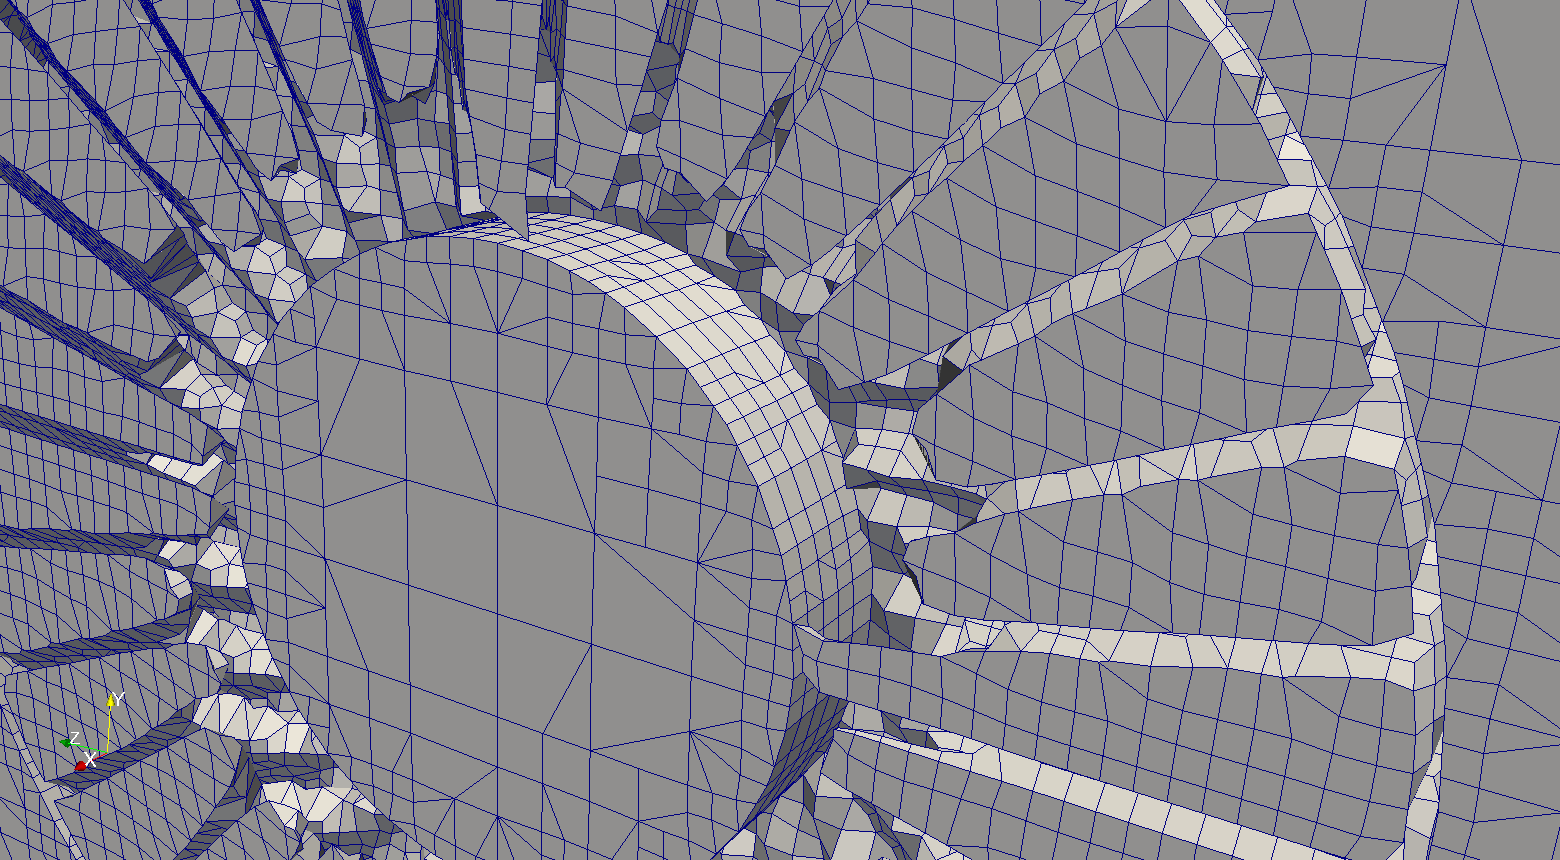
\includegraphics[scale=0.24]{./mesh/screenshots/coarse3}
\centering
\caption{Detail of the coarse mesh}
\label{coarse2}
\end{figure}

\newpage\subsubsubsection{Standard mesh}

\paragraph{}Next, it is presented the standard mesh. It has a higher number of cells compared to the coarse mesh, but it cannot be used either given that the size of the turbine is pretty big. The figures \ref{standard1} and \ref{standard2} are a proof of that.

\begin{figure}[h!]
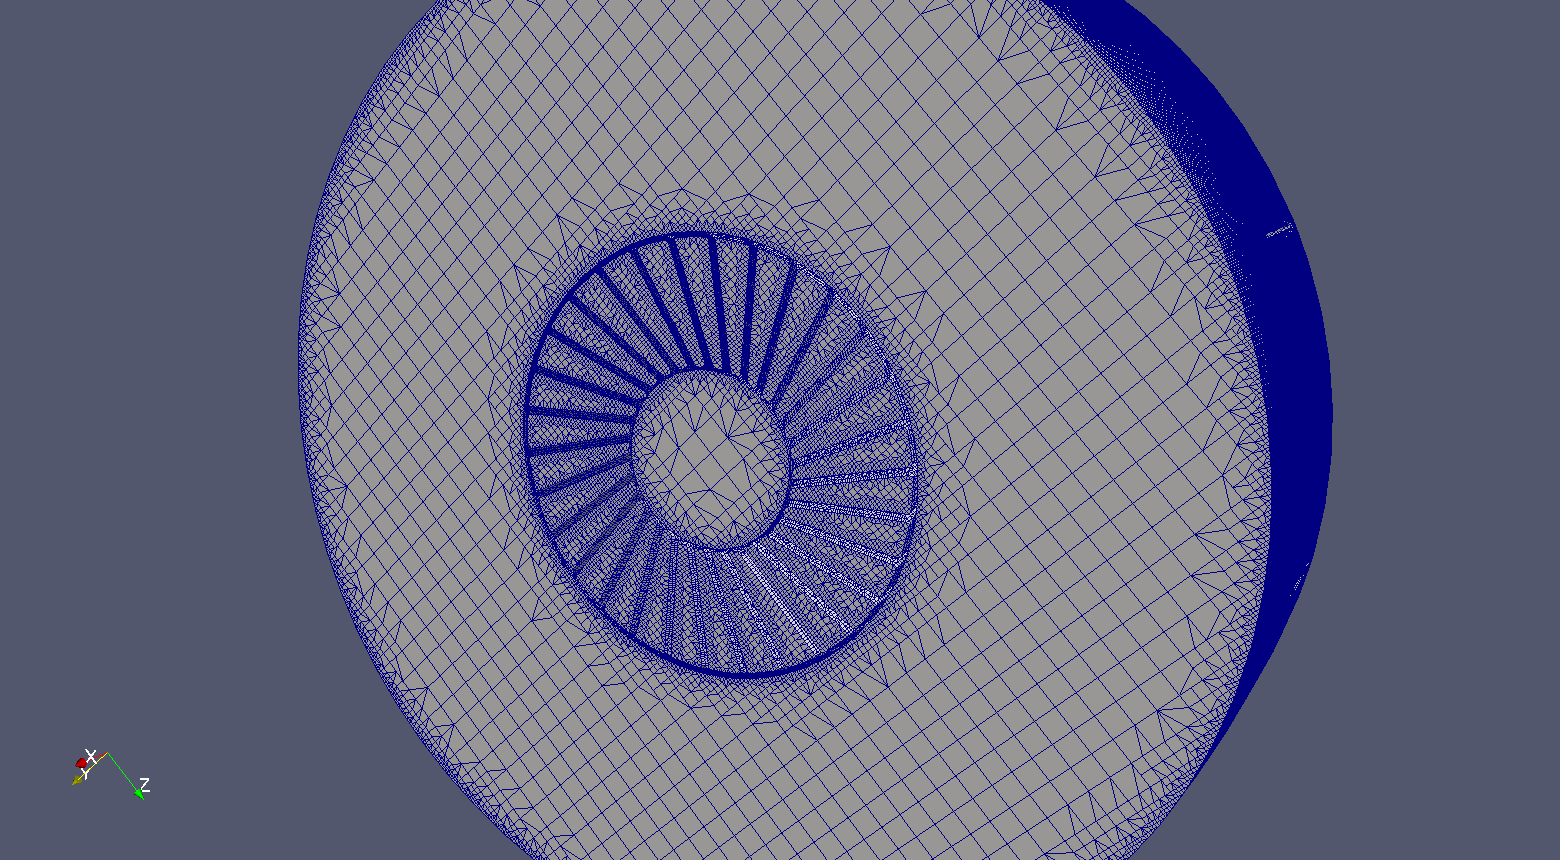
\includegraphics[scale=0.24]{./mesh/screenshots/std2}
\centering
\caption{Detail of the standard mesh}
\label{standard1}
\end{figure}

\begin{figure}[h!]
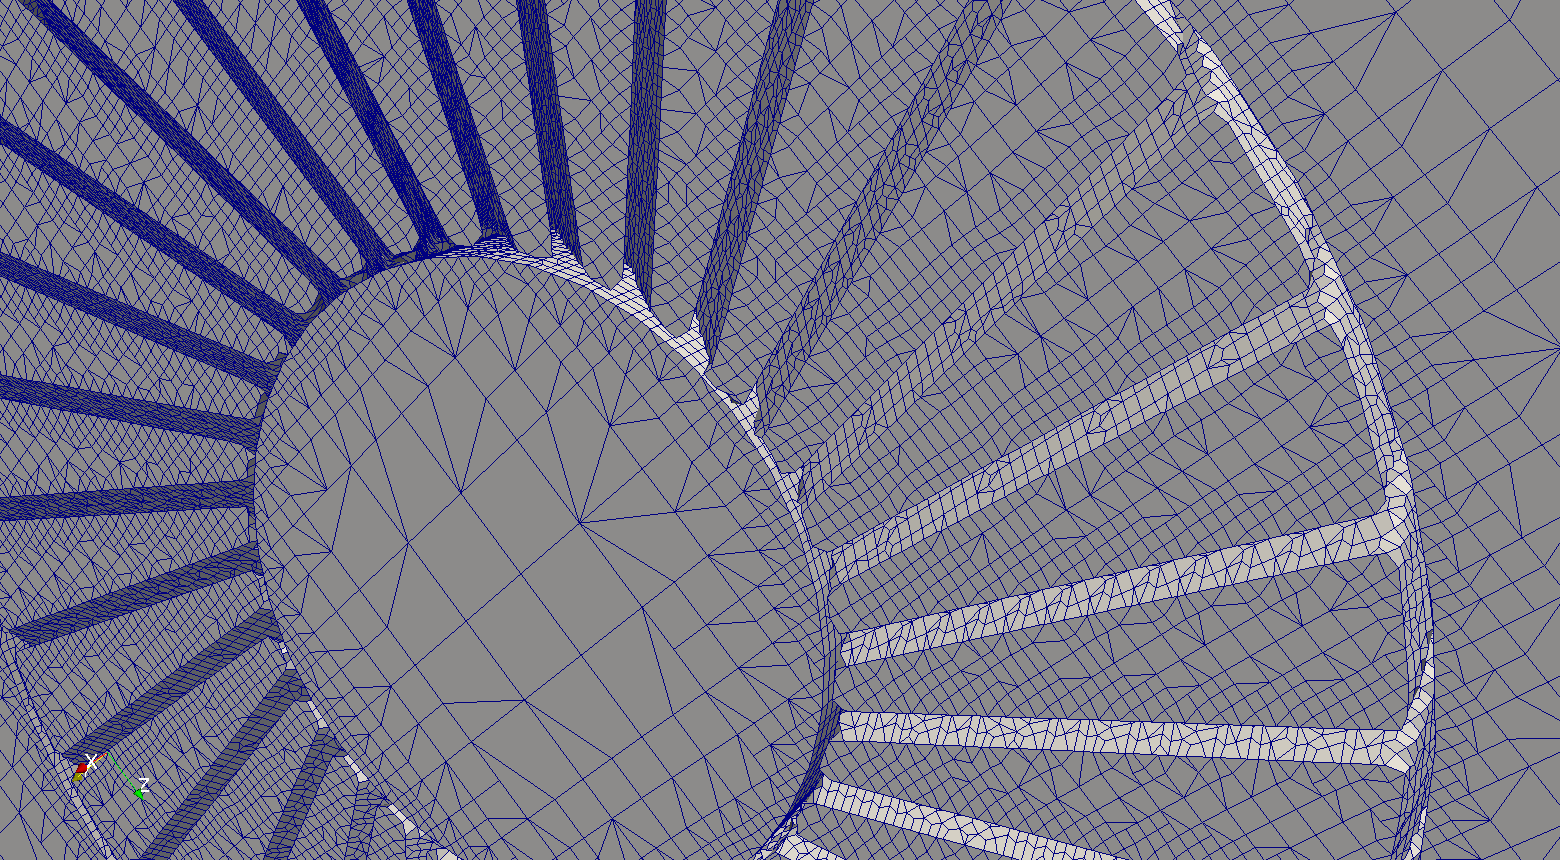
\includegraphics[scale=0.24]{./mesh/screenshots/std3}
\centering
\caption{Detail of the standard mesh}
\label{standard2}
\end{figure}

\newpage\subsubsubsection{Dense mesh}

\paragraph{}Finally, the dense mesh is presented. This is by far the best mesh that has been generated for the case. It can be clearly seen on \ref{dense2} and \ref{dense3}  that it can be suitable to run the simulation of the first stages of this turbofan.


%\begin{figure}[h!]
%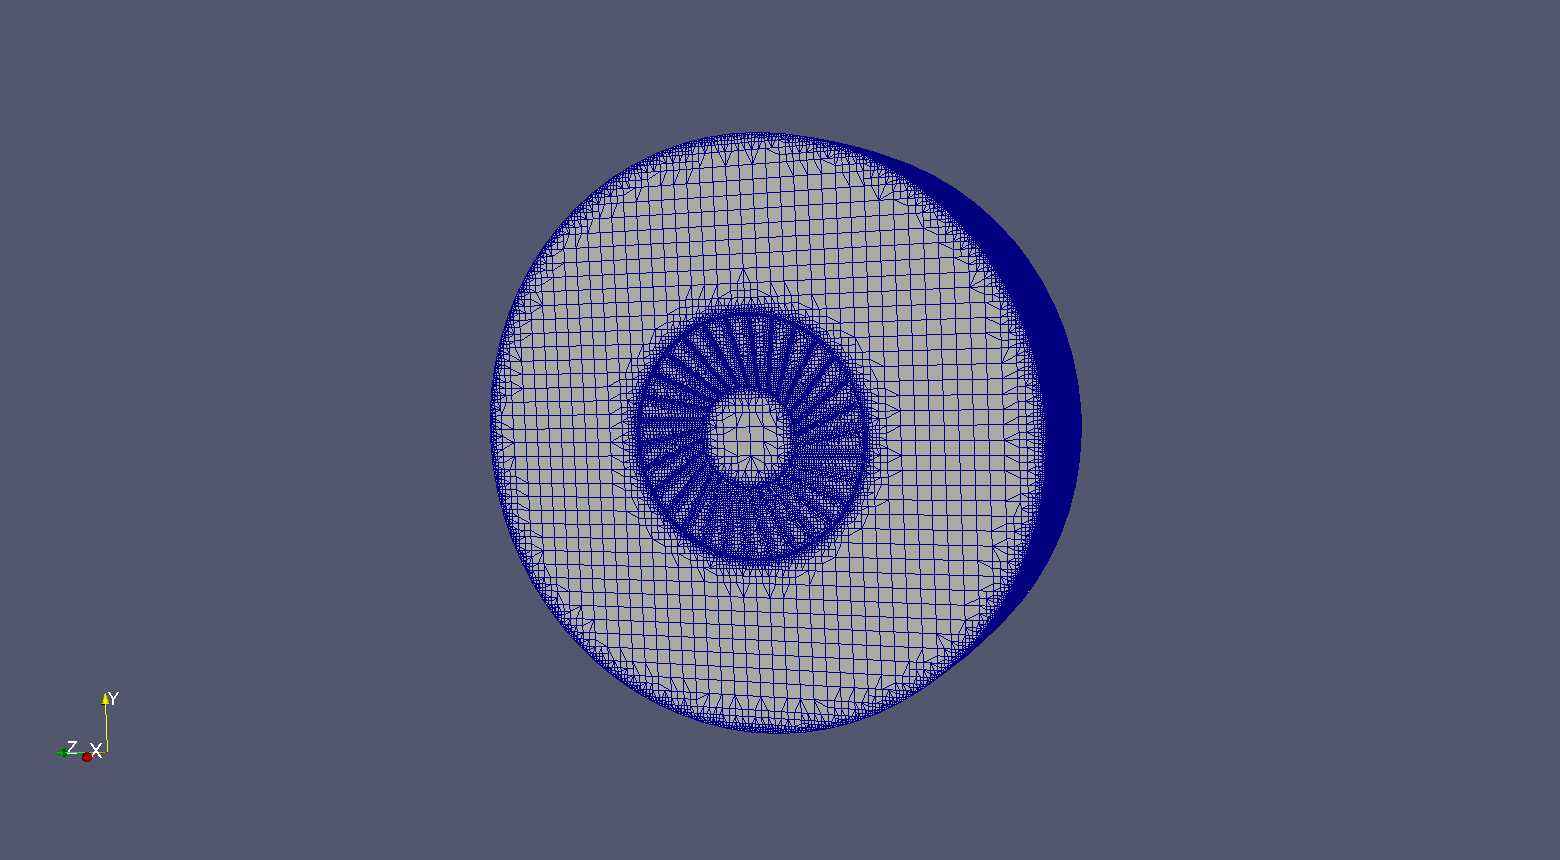
\includegraphics[scale=0.26]{./mesh/screenshots/Xtreme1}
%\centering
%\caption{Detail of the dense mesh}
%\label{dense1}
%\end{figure}

\begin{figure}[h!]
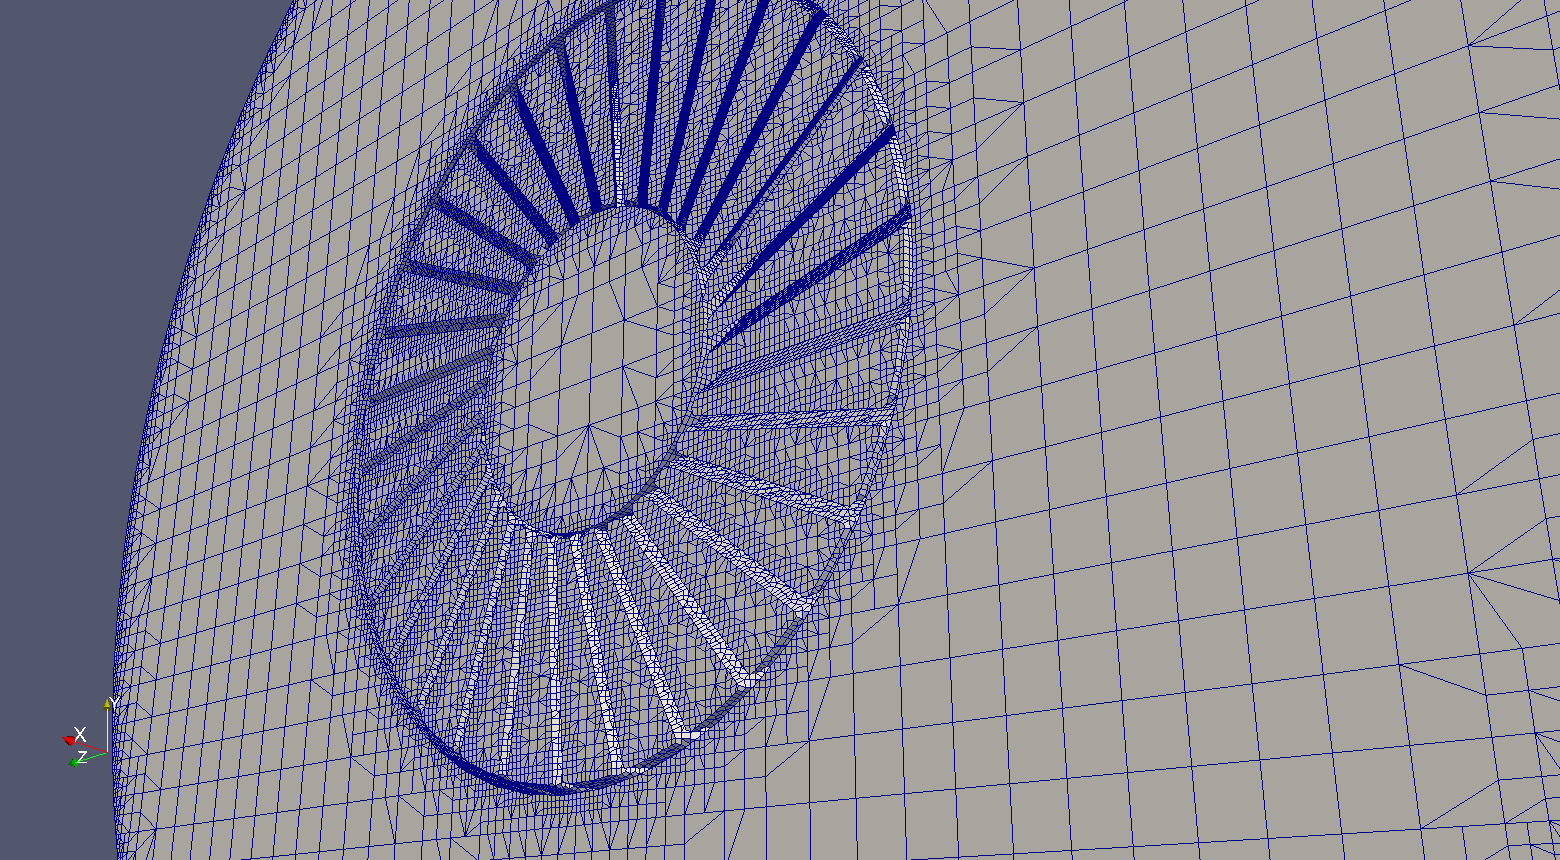
\includegraphics[scale=0.24]{./mesh/screenshots/Xtreme3}
\centering
\caption{Detail of the dense mesh}
\label{dense2}
\end{figure}

\begin{figure}[h!]
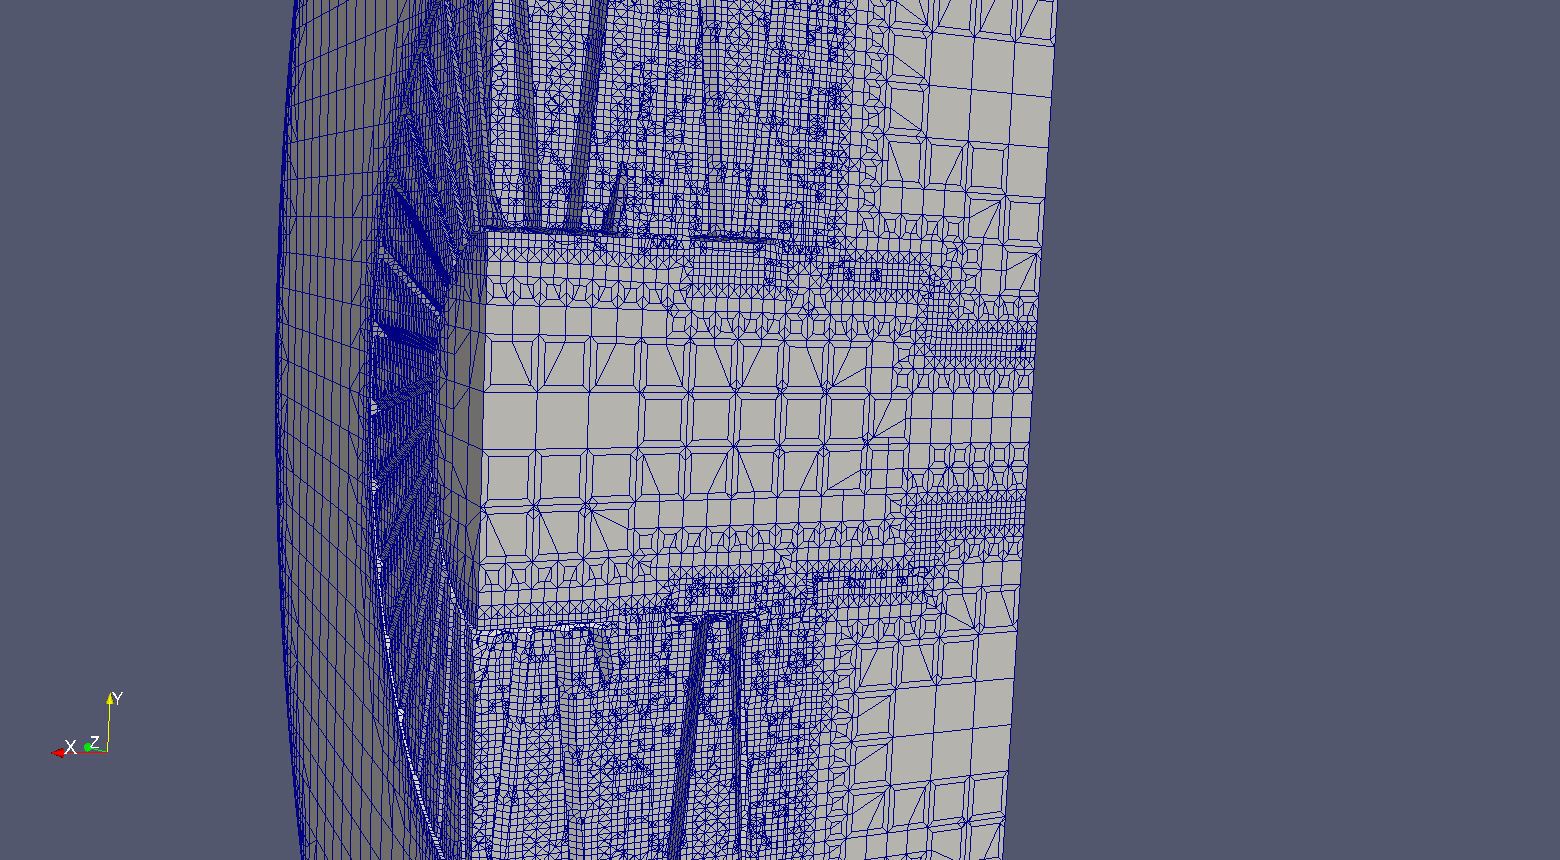
\includegraphics[scale=0.24]{./mesh/screenshots/Xtreme5}
\centering
\caption{Detail of the dense mesh}
\label{dense3}
\end{figure}

\paragraph{}To end with this section, the \textit{log} file that has been obtained when the mesh has been defined with the \textit{snappyHexMesh} utility is presented below. It has to be taken into account that it is a huge file since the number of iterations is really big and only the final part of the \textit{log} file is shown.

\begin{footnotesize}
\begin{verbatim}
Snapped mesh : cells:1626270  faces:5479413  points:2344680
Cells per refinement level:
    0	8592
    1	24456
    2	126790
    3	918976
    4	299109
    5	118950
    6	129397
Writing mesh to time constant
Wrote mesh in = 97.48 s.
Mesh snapped in = 1121.77 s.
Checking final mesh ...
Checking faces in error :
    non-orthogonality > 65  degrees                        : 0
    faces with face pyramid volume < 1e-13                 : 0
    faces with face-decomposition tet quality < 1e-15      : 0
    faces with concavity > 80  degrees                     : 0
    faces with skewness > 4   (internal) or 20  (boundary) : 0
    faces with interpolation weights (0..1)  < 0.05        : 0
    faces with volume ratio of neighbour cells < 0.01      : 0
    faces with face twist < 0.02                           : 0
    faces on cells with determinant < 0.001                : 0
Finished meshing without any errors
Finished meshing in = 1705 s.
End
\end{verbatim}
\end{footnotesize}